\documentclass{beamer}
\usepackage{graphicx}
\usepackage{paralist}
\usepackage{outlines}

\title{Colour Replacement}
\author{Mendocino College - Digital Image Manipulation with Photoshop}
\titlegraphic{\vspace{-10mm}
\includegraphics[width = .9\textwidth]{images/photoshop.jpg}} 
\date{\vspace{-5em}} 


\mode <presentation>
\usetheme{Warsaw}
\usecolortheme{default}

\setbeamerfont{footline}{size=\fontsize{5}{8}\selectfont}

\definecolor{darkred}{rgb}{20,0,0}
\definecolor{darkgreen}{RGB}{40,110,20}
\definecolor{darkpurple}{RGB}{30,0,30}
\definecolor{chardonnay}{RGB}{255, 255, 204}

\setbeamercolor*{palette primary}{fg=white, bg=darkgreen}


\begin{document}
	{
		\setbeamertemplate{footline}{} 
		\setbeamertemplate{headline}{} 
		\begin{frame}
			\vspace{-35pt}
			\maketitle
		\end{frame}
	}

		\section{Design Principles}
			\subsection{Design Principles}		
			\begin{frame}
				\frametitle{Design Principles}
				\begin{columns}
					\column{.6\textwidth}
					\vspace{-25pt}
					\begin{outline}
						\1 Design principles are general guidelines for how to put together elements in a piece to make it visually interesting, aesthetic, or effective. These guidelines can be modified to accomplish the purpose of the designer.
						\1 In Graphic Design there are 8 basic principles for design.
						\1 We are going to focus on 10 design principles for photographers
					\end{outline}
					\column{.45\textwidth}
					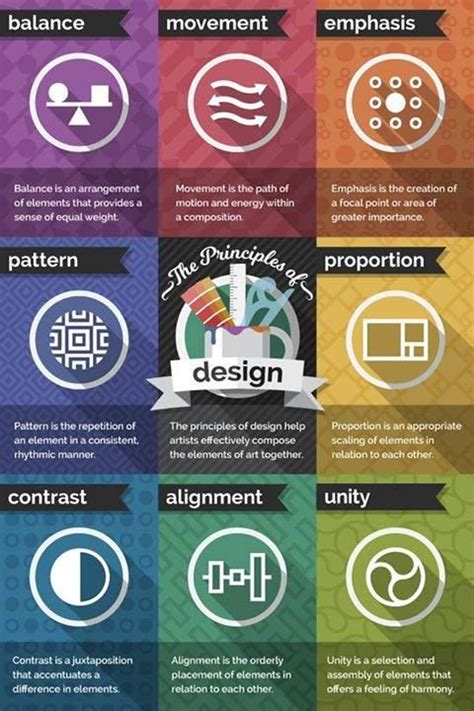
\includegraphics[width=0.9\textwidth]{images/principles of design.jpeg}
				\end{columns}
			\end{frame}

		\section{8 Basic Design Principles}
\subsection{8 Basic Design Principles}		
\begin{frame}
	\frametitle{Balance, Movement, \& Emphasis}
		\begin{outline}
			\1 Balance – 
			\2 the concept of visual equilibrium. Like items on a scale, each item has a certain visual weight and these weights should balance. For example, vibrant color has more visual weight than muted color. Balance is further described below under photographic design principles.
			\1 Movement - 
			\2 can be described as timed movement through space; an easy, connected path that the eye follows through the composition. The presence of rhythm creates predictability and order.
			\1 Emphasis - 
			\2 it is also referred to as dominance or focal point. It marks the location(s) in a composition that most strongly draw the viewer's attention by providing some visual "surprises". It is also one of our photographic design principles.
		\end{outline}
\end{frame}

\begin{frame}
	\frametitle{Pattern, Proportion, \& Contrast}
	\begin{outline}
		\1 Pattern - 
		\2 The Repetition of an element in a consistent, rhythmic manner.
		\1 Proportion - 
		\2 The relative size and scale of the various elements in a design. It adds interest when the elements are out of proportion. I would consider it a subset of the contrast principle.
		\1 Contrast - 
		\2 The juxtaposition that accentuates a difference in elements.
	\end{outline}
\end{frame}

\begin{frame}
	\frametitle{Alignment \& Unity}
	\begin{outline}
		\1 Alignment - 
		\2 The orderly placement of elements in relation to each other.
		\1 Unity - 
		\2 the underlying principle that encompasses many of the principles and elements of design. It refers to the coherence of the whole, the sense that all of the parts are working together to achieve a common result; a harmony of all the parts.
	\end{outline}
\end{frame}

		\section{10 Photographers Design Principles}
\subsection{10 Photographers Design Principles}		
\begin{frame}
	\frametitle{Framing, Angle of View, Emphasis, and Contrast}
	\begin{outline}
		\1 Framing – 
		\2 it doesn’t necessarily mean that there is something in the image that literally frames the content, such as looking out through an open door. It means that the photograph has an interesting composition without distracting elements. Often there is a compelling person or object in the foreground.
		\1 Angle of view - 
		\2 the idea here is to show the item from a perspective that is unusual and therefore interesting.
		\1 Emphasis - 
		\2 Note that it’s all about a strong focal point. The viewer’s eye should be immediately drawn to that item
				\1 Contrast - 
		\2 makes the photograph more interesting by including elements that are dramatically different in tone, color, size, lines, or texture. Similar to Emphasis, but does not create a focal point.
	\end{outline}
\end{frame}

\begin{frame}
	\frametitle{Rule of Thirds and Close Ups}
	\begin{outline}
		\1 Rule of thirds – 
		\2 within the image, draw two evenly-spaced horizontal lines and two evenly-spaced vertical lines. The main item of interest, such as the center of someone’s face, should be located at one of the four intersections or along one of those lines. Another application is for one or more major elements to take up a third of the image. For example, in an image with a horizon, two-thirds of the image should be sky if the clouds or sunset is more interesting and two-thirds of the image should be the ground if the landscape is more interesting
		\1 Close Ups - 
		\2 like Angle of view, we want to show an item in a way that it is not normally seen. I find the examples in the textbook to be only marginally close up. A better example would be an ant taking up the full frame.
	\end{outline}
\end{frame}

\begin{frame}
	\frametitle{Balance, \& Line and Shape}
	\begin{outline}
		\1 Balance – 
		\2 the visual weight of items are balanced across the image like two people on a see-saw. The following can be used to achieve balance or visual weight:
		\3 Several small or light shapes to counterbalance a large or dark shape
		\3 Textures with darker values to counterbalance a lightly textured surfaces with lighter values
		\3 Shapes placed above eye level add more visual weight
		\3 Irregular shapes are usually heavier than more easily-recognized shapes
		\3 Lines placed close together. They will appear darker and can help counterbalance a dark solid mass.
		\1 Line and shape - 
		\2 the viewer’s eye tends to follow lines and pause on recognizable shapes. Related to the Emphasis design principle.
	\end{outline}
\end{frame}

\begin{frame}
	\frametitle{Balance, \& Line and Shape}
	\begin{outline}
		\1 Tone and sharpness – 
		\2 lighter and sharper objects also draw the eye. Photographers use a narrow depth of field (wide lens aperture) so that only the object in the foreground is in focus. This effect can be easily duplicated in Photoshop.
		\1 Arrangement - 
		\2 keep it simple and uncluttered.
		\1 Rule of Odds - 
		\2 suggests that an odd number of subjects in an image is more interesting than an even number. For example in artwork, frame an object of interest with an even number of surrounding objects.
		\3 This is not an actual rule, but a suggestion.
	\end{outline}
\end{frame}
	
	
\end{document}